% Architecture Layers Diagram for OpenRoad-GUI
% Compile standalone with: pdflatex architecture_layers.tex
% Then include as: 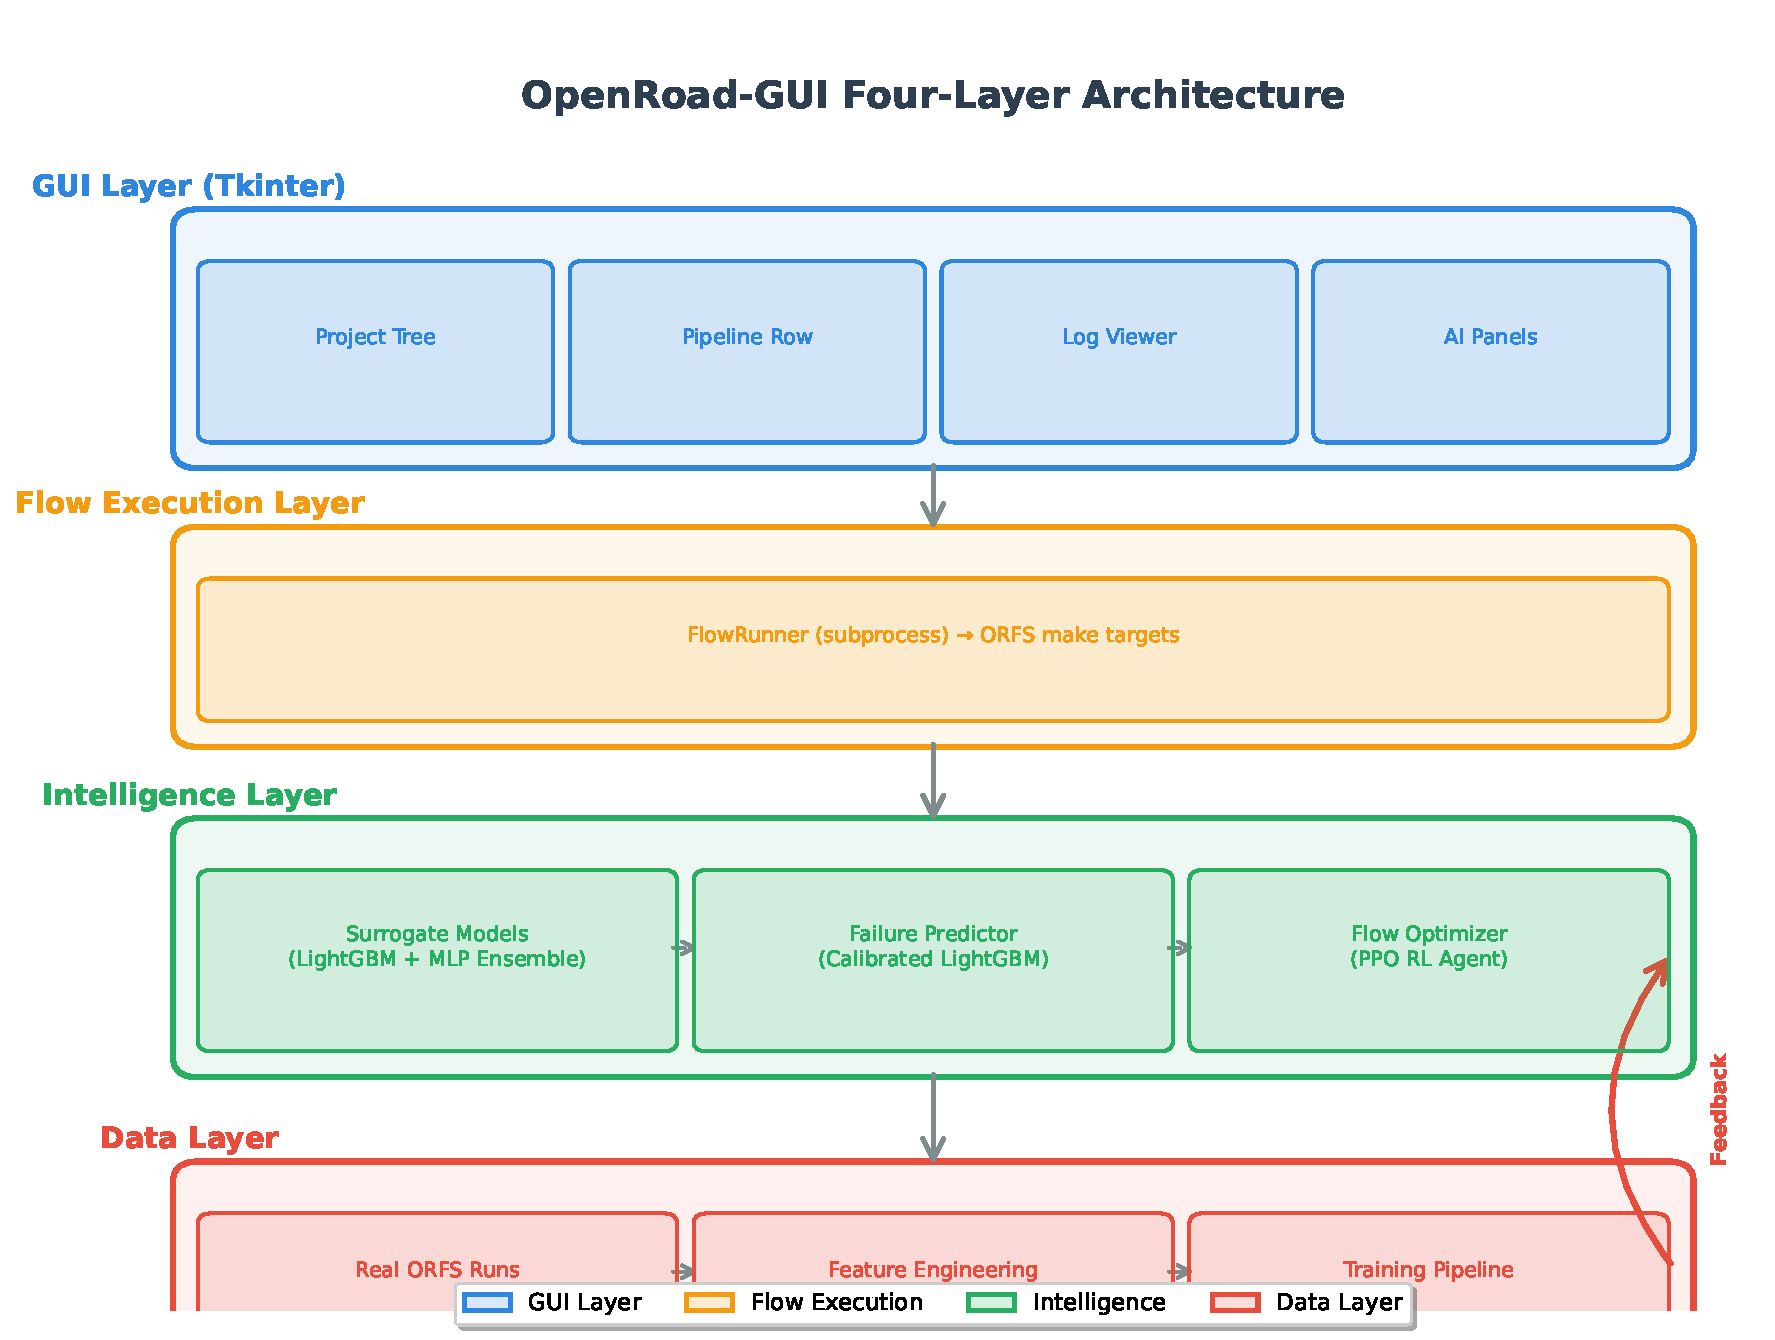
\includegraphics{figures/architecture_layers.pdf}

\documentclass[tikz,border=10pt]{standalone}
\usepackage{tikz}
\usetikzlibrary{positioning, shapes, arrows.meta, shadows, fit, backgrounds}

\begin{document}

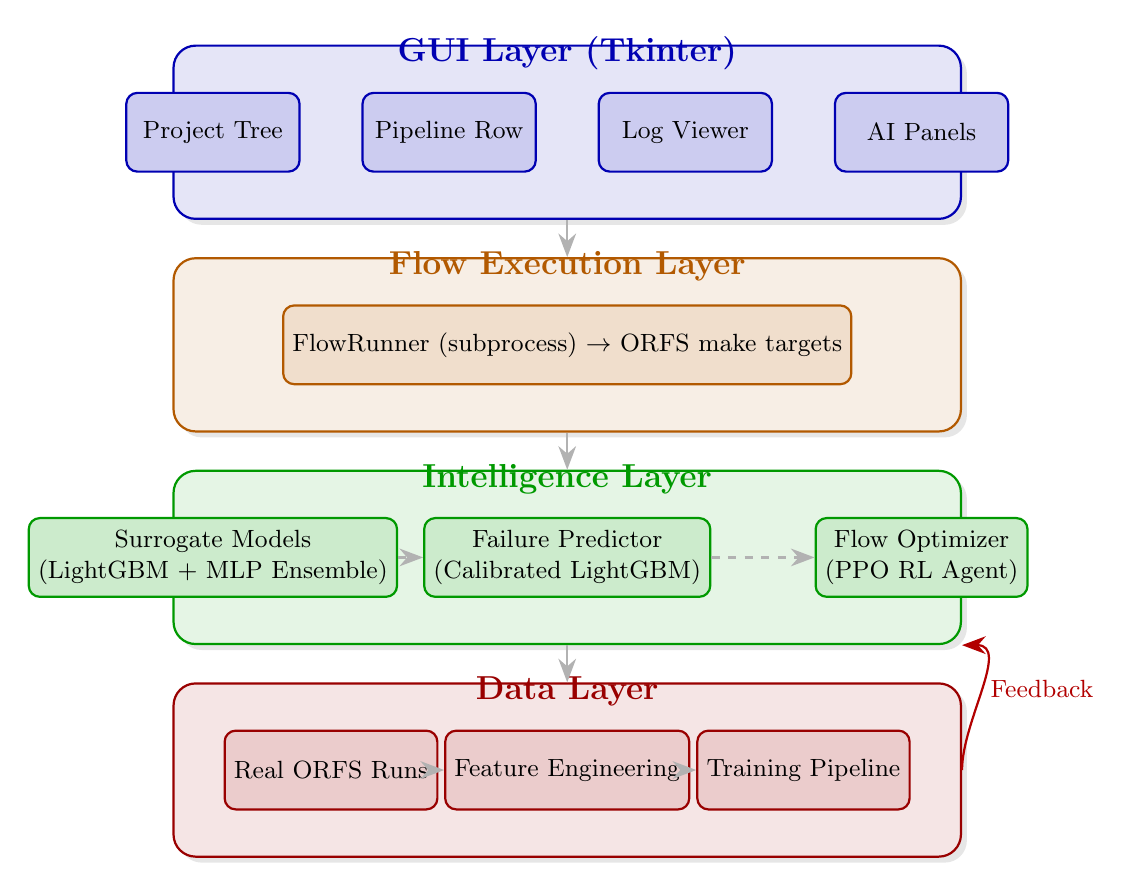
\begin{tikzpicture}[
    node distance=1.2cm and 2cm,
    layer/.style={
        rectangle,
        rounded corners=8pt,
        minimum width=10cm,
        minimum height=2.2cm,
        draw=#1,
        thick,
        fill=#1!10,
        drop shadow={opacity=0.2},
        align=center
    },
    component/.style={
        rectangle,
        rounded corners=4pt,
        minimum width=2.2cm,
        minimum height=1cm,
        draw=#1,
        thick,
        fill=#1!20,
        font=\small,
        align=center
    },
    arrow/.style={
        -{Stealth[length=3mm]},
        thick,
        draw=gray!60
    },
    title/.style={
        font=\bfseries\large,
        text=#1
    }
]

% Layer 1: GUI Layer (top)
\node[layer=blue!70!black] (gui) at (0, 5.5) {};
\node[title=blue!70!black] at (0, 6.5) {GUI Layer (Tkinter)};
\node[component=blue!70!black] (gui1) at (-4.5, 5.5) {Project Tree};
\node[component=blue!70!black] (gui2) at (-1.5, 5.5) {Pipeline Row};
\node[component=blue!70!black] (gui3) at (1.5, 5.5) {Log Viewer};
\node[component=blue!70!black] (gui4) at (4.5, 5.5) {AI Panels};

% Layer 2: Flow Execution Layer
\node[layer=orange!70!black] (flow) at (0, 2.8) {};
\node[title=orange!70!black] at (0, 3.8) {Flow Execution Layer};
\node[component=orange!70!black] (flow1) at (0, 2.8) {FlowRunner (subprocess) $\rightarrow$ ORFS make targets};

% Layer 3: Intelligence Layer
\node[layer=green!60!black] (intel) at (0, 0.1) {};
\node[title=green!60!black] at (0, 1.1) {Intelligence Layer};
\node[component=green!60!black] (intel1) at (-4.5, 0.1) {Surrogate Models\\(LightGBM + MLP Ensemble)};
\node[component=green!60!black] (intel2) at (0, 0.1) {Failure Predictor\\(Calibrated LightGBM)};
\node[component=green!60!black] (intel3) at (4.5, 0.1) {Flow Optimizer\\(PPO RL Agent)};

% Layer 4: Data Layer (bottom)
\node[layer=red!60!black] (data) at (0, -2.6) {};
\node[title=red!60!black] at (0, -1.6) {Data Layer};
\node[component=red!60!black] (data1) at (-3, -2.6) {Real ORFS Runs};
\node[component=red!60!black] (data2) at (0, -2.6) {Feature Engineering};
\node[component=red!60!black] (data3) at (3, -2.6) {Training Pipeline};

% Arrows between layers
\draw[arrow] (gui.south) -- ++(0,-0.3) -| (flow.north);
\draw[arrow] (flow.south) -- ++(0,-0.3) -| (intel.north);
\draw[arrow] (intel.south) -- ++(0,-0.3) -| (data.north);

% Internal arrows in Intelligence Layer
\draw[arrow, dashed] (intel1.east) -- (intel2.west);
\draw[arrow, dashed] (intel2.east) -- (intel3.west);

% Internal arrows in Data Layer
\draw[arrow] (data1.east) -- (data2.west);
\draw[arrow] (data2.east) -- (data3.west);

% Feedback loop from Data to Intelligence
\draw[arrow, bend right=40, red!70!black, thick]
    (data.east) to[out=0, in=-90]
    node[right, midway, font=\small, text=red!70!black] {Feedback}
    (intel.south east);

\end{tikzpicture}

\end{document}